\subsection{Physical layer}

Physical layer is the first layer of the \acrshort{osi} reference model. The main role of the physical layer is a transmission of electrical, optical or radio signal over transmission medium. This layer describes the transmission medium itself (whether it is metallic or optical cable, wireless, etc.) and its properties, network interface parameters and nature of transmitted signal; in other words, physical properties and characteristics of a transmitted signal and a transfer medium. The physical layer does not understand transmitted data itself, it only sees it as a stream of bits and is responsible for their transmission. It provides service to the Data link layer.

Main functions and services offered by this layer are:
\begin{itemize}[noitemsep]
    \item Establishing and termination of connection with communication medium
    \item Modulation or conversion of digital data from the user’s device to the corresponding signals transmitted by the communication channel
    \item Physical topology
    \item Transmission mode and rate
    \item Physical characteristics
    \item Bit representation
\end{itemize}

Components of physical layer may be divided into passive and active components. Active components are those that amplify or modify a transmitted signal. The most common devices are transceivers or repeaters. Passive components, unlike active ones, do only transmit a signal and do not modify, amplify or create it in any way, for example cables or connectors.

In case of IoT and \acrfull{wsn}, data are transmitted wirelessly and wireless networks as well as their physical layer have different characteristics to wired ones. To be able to send any kind of information or data over the air, there must be a certain portion of the radio spectrum allocated for this purpose. As it may be seen in~\ref{fig:freq-alloc}, the radio spectrum is already very crowded, so this resource is very sacred. Most of the spectrum’s frequency bands are already given their use for different purposes like TV signal transmission, FM radio or maritime communication. Therefore, if a new technology emerges and would like to use a frequency band of the spectrum, it can either pay and get a licensed band or can use special license-free bands like ISM radio band (industrial, scientific and medical) or U-NII band, which may be used freely. That is what most physical layer protocols does, make use of a freely available bands, which makes a technology cheaper, but the interference is higher as the band is more crowded.

\begin{figure}[ht]
    \centering
    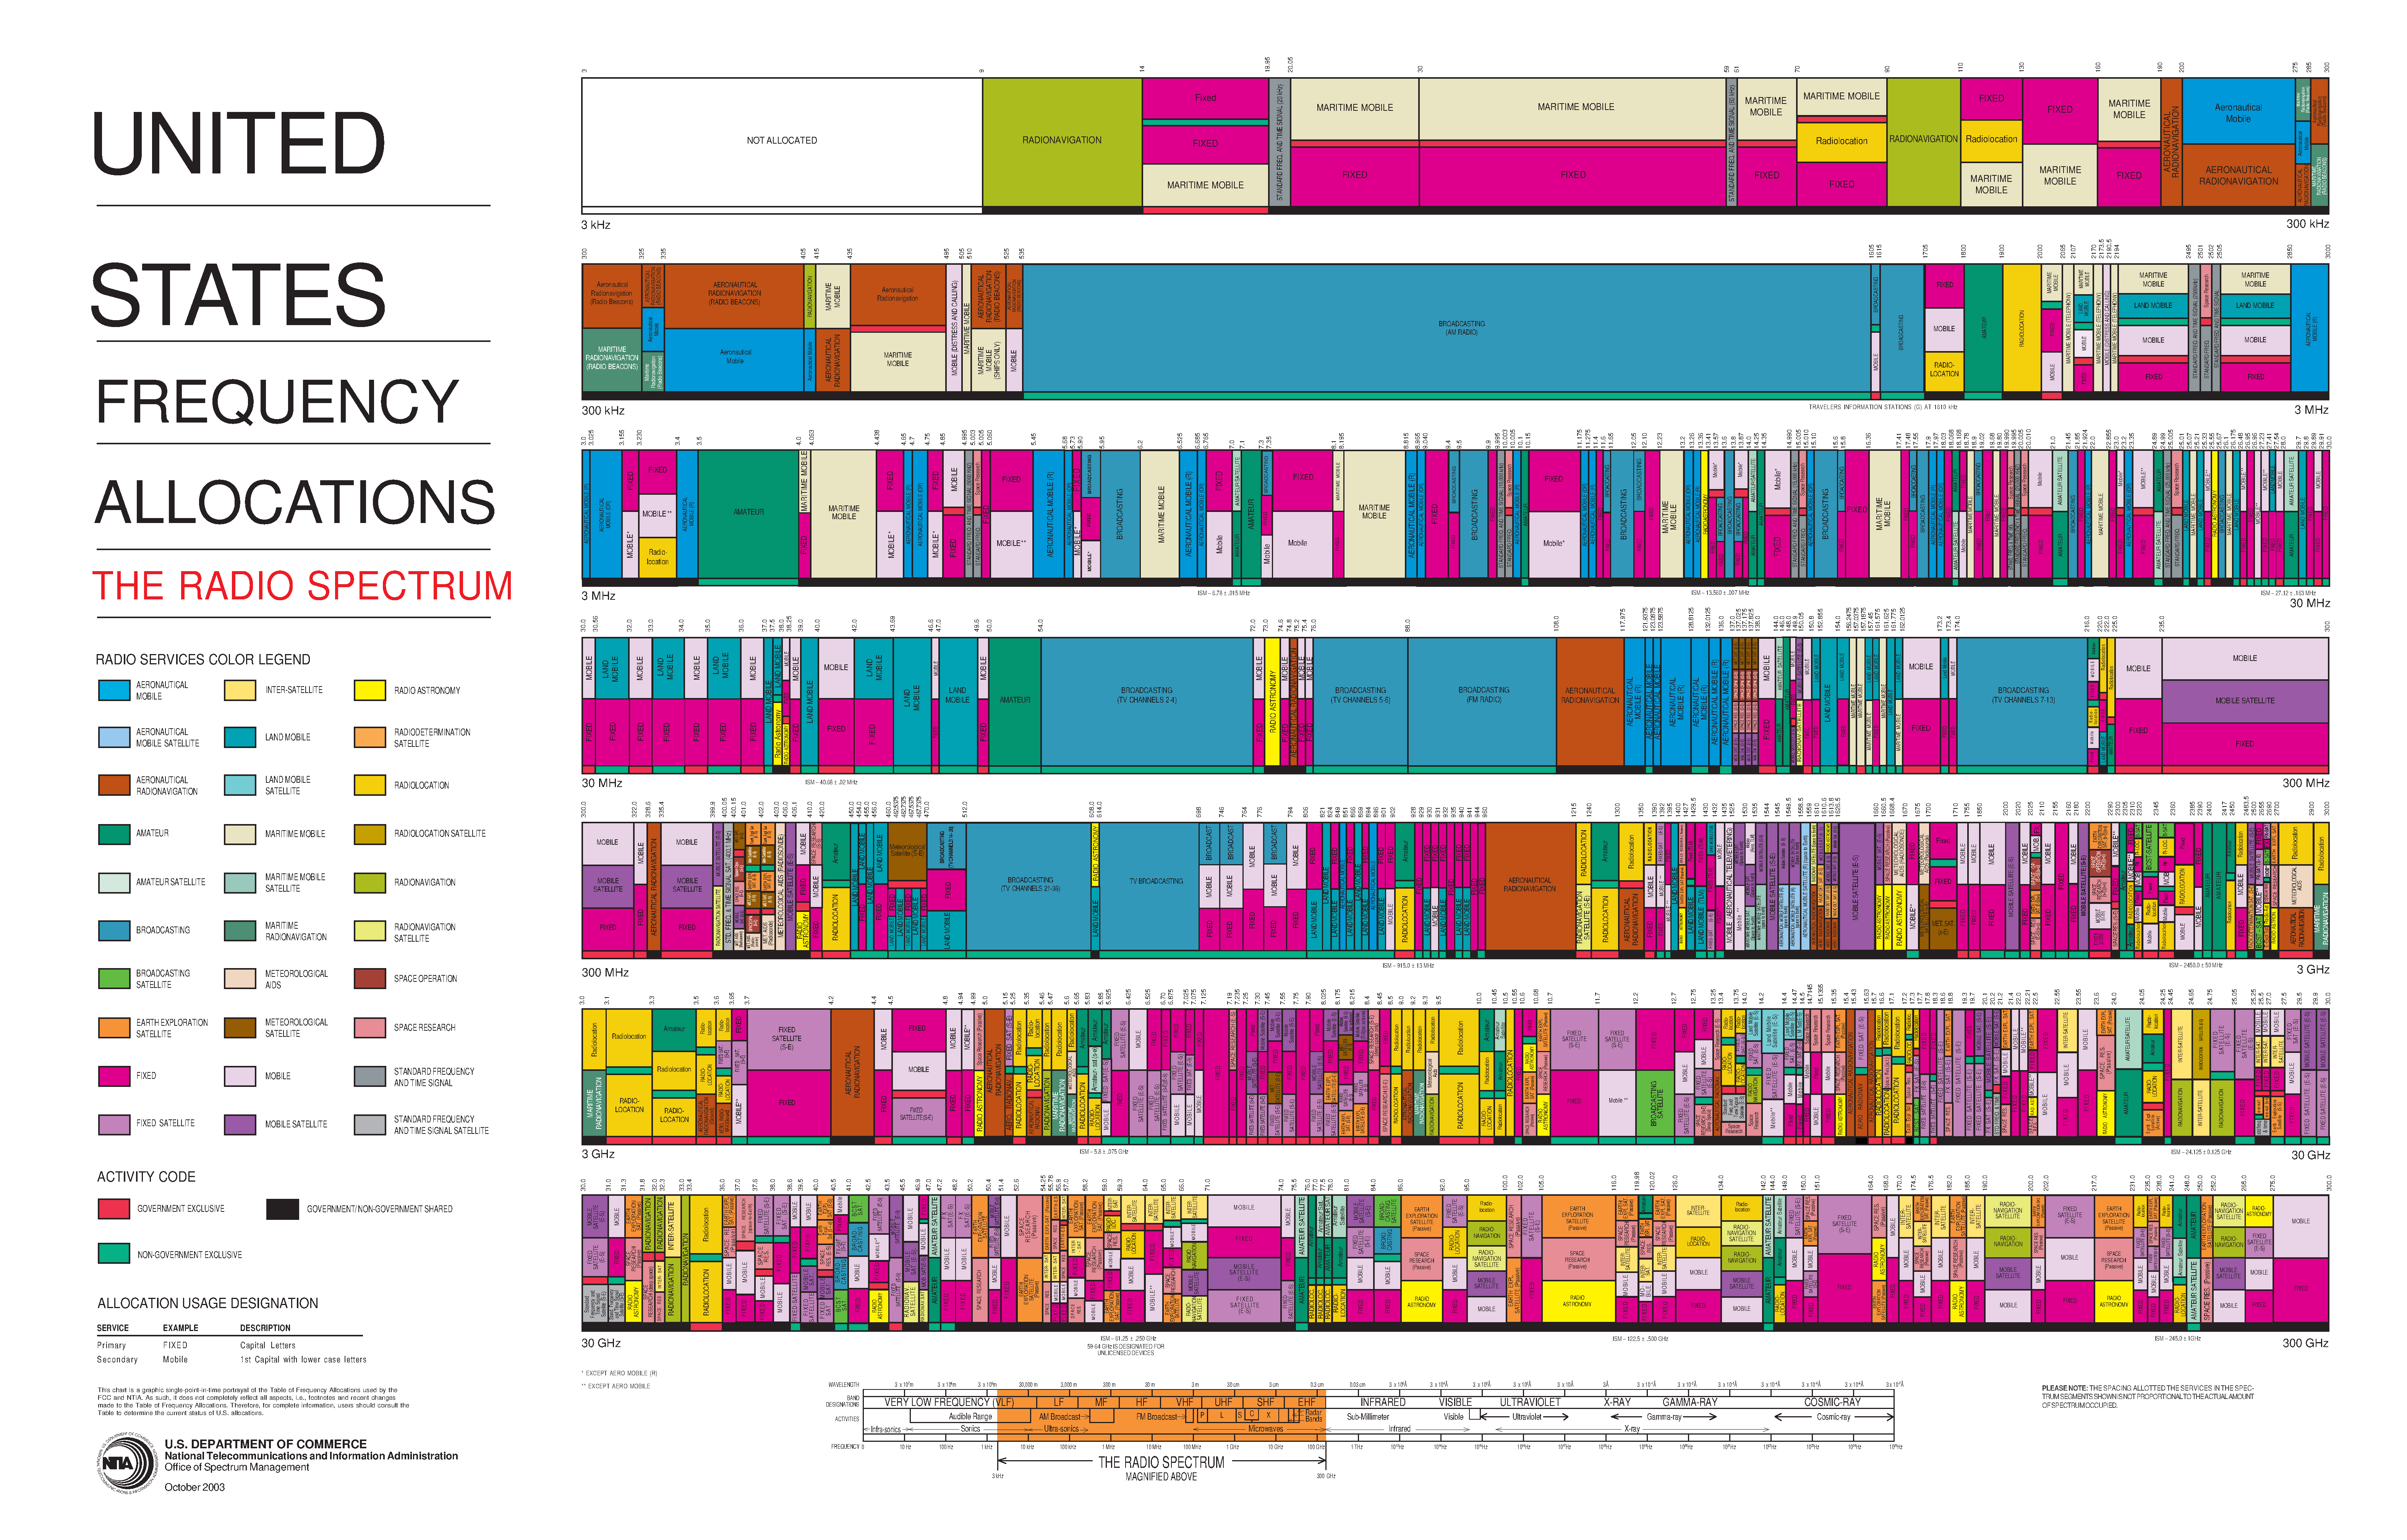
\includegraphics[width=\textwidth]{00images/freq-alloc}
    \caption{Example of how radio spectrum is crowded in United States and for which use are frequencies of the spectrum allocated. Source: \url{https://www.ntia.doc.gov/files/ntia/publications/2003-allochrt.pdf}, accessed 11-05-2018}
    \label{fig:freq-alloc}
\end{figure}

Spectral efficiency says how much of an information can be send over a given portion of frequency spectrum, how well the frequency spectrum is utilised. This is important in wireless networks, as frequency bands are limited and the higher the utilisation the better. Another important aspect of wireless transmission is the range. Unlike in wired communication where interference in cables is low (isolated cables), so bandwidth may be high (modulation techniques) and long cables used, wireless communication suffers from interference, lower bandwidth and propagation loss a lot. As it may be seen in~\ref{fig:radio-spectrum}, choosing the right frequency band is crucial, because the lower frequencies have higher range, devices are cheaper to produce, but bandwidth is smaller while the higher the frequency band, the higher the bandwidth but smaller the range. On top of that, \acrshort{iot} devices are many times battery powered, meaning they must be power efficient and a ration between signal strength, power consumption and bandwidth must be chosen carefully.

\begin{figure}
    \centering
    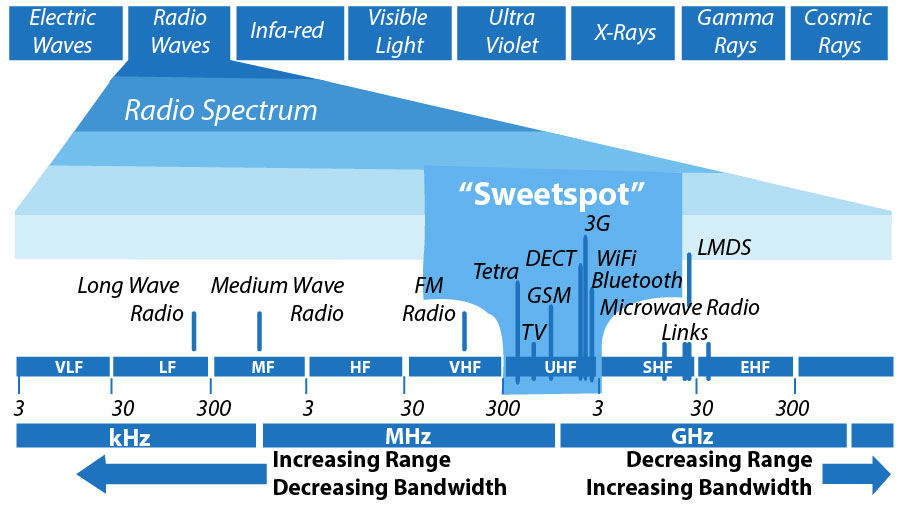
\includegraphics[width=0.8\textwidth]{00images/radio-spectrum-3}
    \caption{Radio spectrum division to frequency groups and the ``sweetspot'' location. Source: \url{https://nuzeal.com/index.php/radio-spectrum-availability/}, accessed 11-05-2018}
    \label{fig:radio-spectrum}
\end{figure}{}
% 
% There are several metrics that can be used to assess the performance of a physical layer. These metrics are listed in Table~\ref{tab:metrics-physical}.
% 
% \begin{table}[ht]
%      \centering
%     \begin{tabularx}{\textwidth}{|l|X|p{5em}|}
%     \hline
%     \textbf{Metrics}&\textbf{Description}&\textbf{Relevance}\\
%     \hline
%     Range&Range is a metrics that tells how far from transmitter may a message be successfully received by a receiver.&••\\
%     Throughput&Throughput is the rate of successful message delivery through the communication channel.&•\\
%     Spectral efficiency&Spectral efficiency tells how much the frequency band is utilised.&•\\
%     Power consumption&Power consumption describes how much power is need by a device to send a message of the same size.&••\\
%     \hline
%     \end{tabularx}
    
%     \caption{Metrics used to evaluate protocols in physical layer.}
%     \label{tab:metrics-physical}
% \end{table}{}
